\section{Reto}
\begin{frame}{Reto}
    \Huge\centering\textbf{CHALLENGE TIME!}
\end{frame}

\subsection{The Legend of Zelda: Phantom Hourglass}
\begin{frame}[t]{Contenido sorpresa}
    \begin{columns}
    \begin{column}[T]{0.5\textwidth}
        \centering
        \visible<2->{¿\textit{/Test/picture.narc}?\\\vspace{5pt}}
        \visible<3->{\includegraphics[width=\textwidth]{imgs/zelda_dog.png}}
    \end{column}
    \hfill
    \begin{column}[T]{0.5\textwidth}
        \centering
        \visible<4->{¿\textit{/Test/BgMap.narc}?\\\vspace{5pt}}
        \visible<5->{\includegraphics[width=0.5\textwidth]{imgs/zelda_batch.png}}
    \end{column}
    \end{columns}
\end{frame}

\begin{frame}{Historia}
    \begin{columns}
    \begin{column}{0.5\textwidth}
        \begin{itemize}
            \item<1-> Modificar cuarto diálogo.
            \item<2-> Modificar imagen.
        \end{itemize}
        \vfill{}
        \visible<3->{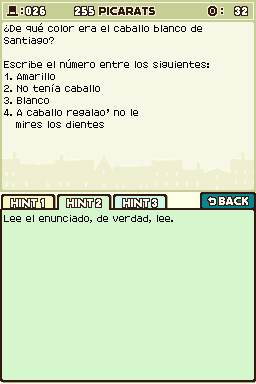
\includegraphics[width=0.4\textwidth]{imgs/reto3.png}}
        \hfill{}
        \visible<4->{\includegraphics[width=0.5\textwidth]{imgs/reto4.png}}
    \end{column}
    \begin{column}{0.5\textwidth}
        \visible<1->{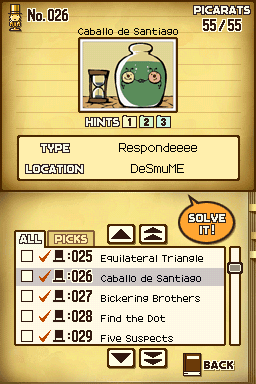
\includegraphics[width=0.4\textwidth]{imgs/reto1.png}}
        \hfill{}
        \visible<2->{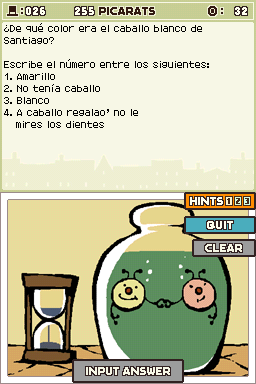
\includegraphics[width=0.4\textwidth]{imgs/reto2.png}}
        \vfill{}
        \begin{itemize}
            \item<3-> Modificar tipografía.
            \item<4-> Modificar mapa.
        \end{itemize}
    \end{column}
    \end{columns}
\end{frame}

\begin{frame}{Historia: Punteros}
    \begin{columns}
    \begin{column}{0.3\textwidth}
        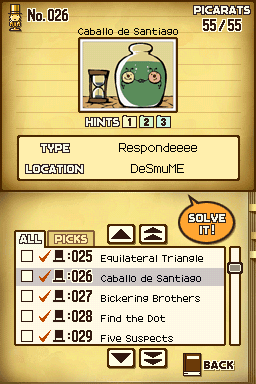
\includegraphics[width=\textwidth]{imgs/reto1.png}
    \end{column}
    \begin{column}{0.7\textwidth}
        Modificar cuarto diálogo.
        \footnotesize
        \begin{itemize}
            \item Ruta: \textit{/Spanish/Message/demo.bmg}.
            \item Punteros en la sección \texttt{INF1} (cabecera: 16 B).
            \item Hay \texttt{0x08} bytes por texto.
            \item Primeros \texttt{0x04} bytes es el puntero.
            \item Puntero \textit{i}: $Offset_{INF1} + 16 + i*8=48h$.
            \item Punteros relativos a \texttt{0x0AE8}.
            \item Ignorar 6 bytes después de \texttt{001Ah}.
            \item Añadir pausa al final con: \\
                  \texttt{1A 00 08 01 0E 00 7D 00}.
        \end{itemize}
    \end{column}
    \end{columns}
\end{frame}

\begin{frame}{Historia: Imágenes}
    \begin{columns}
    \begin{column}{0.7\textwidth}
        Modificar imagen
        \footnotesize
        \begin{wideitemize}
            \item Ruta: \textit{/Event/Kamishibai/kami1/kami1-01}.
            \item Seleccionar \textit{Replace palette}.
            \item Importar imagen con mismas dimensiones:
            \begin{itemize}
                \item Ancho: \texttt{256} píxeles.
                \item Alto: \texttt{192} píxeles.
            \end{itemize}
        \end{wideitemize}
    \end{column}
    \begin{column}{0.3\textwidth}
        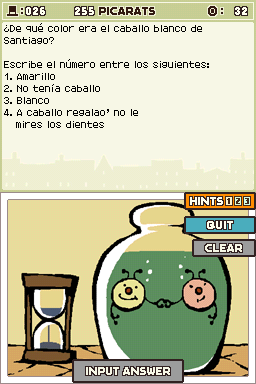
\includegraphics[width=\textwidth]{imgs/reto2.png}
    \end{column}
    \end{columns}
\end{frame}

\begin{frame}{Historia: Tipografía}
    \begin{columns}
    \begin{column}{0.3\textwidth}
        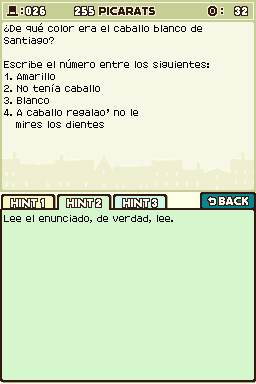
\includegraphics[width=\textwidth]{imgs/reto3.png}
    \end{column}
    \begin{column}{0.7\textwidth}
        Modificar tipografía
        \footnotesize
        \begin{wideitemize}
            \item Cambiar primer texto por:\\
                  $\int2x dx=x^2+K$
            \item Tipografía: \textit{/Font/zeldaDS\_15.nftr}.
            \item Reemplazar caracteres japoneses por: $\int$ y $^2$
        \end{wideitemize}
    \end{column}
    \end{columns}
\end{frame}

\begin{frame}{Mapas}
    \begin{columns}
    \begin{column}{0.7\textwidth}
        Modificar mapa
        \footnotesize
        \only<1-5>{
        \begin{wideitemize}
            \item Ruta: \textit{/Map/isle\_main/}
            \item<2-> \textit{course.bin}: texturas del mapa.
            \item<3-> \textit{map00.bin}: mapa principal.
            \begin{itemize}
                \footnotesize
                \item<4-> \textit{isle\_main\_00.nsbmd}: terreno 3D.
                \item<5-> \textit{isle\_main\_00.zmb}: Mapa de colisiones y objetos.
            \end{itemize}
        \end{wideitemize}
        }
        \only<6->{
        \begin{itemize}
            \item<6-> Sección \texttt{BMOR}: mapa de colisiones.
            \item<7-> Sección \texttt{PRAW}: salidas del mapa.
            \item<8-> Sección \texttt{BOPM}: objetos del terreno:
            \begin{itemize}
                \footnotesize
                \item<8-> \texttt{0x1C} bytes por objeto.
                \item<8-> Primeros dos bytes: tipo de objeto.
                \item<8-> Siguientes dos bytes: posición X e Y.
            \end{itemize}
        \end{itemize}
        }
    \end{column}
    \begin{column}{0.3\textwidth}
        \only<1-3>{\includegraphics[width=\textwidth]{imgs/reto4.png}}
        \only<4-5>{\includegraphics[width=\textwidth]{imgs/zelda_map.png}}
        \only<6->{\includegraphics[width=\textwidth]{imgs/reto4_1.png}}
    \end{column}
    \end{columns}
\end{frame}
